In this section, we evaluate performance of dxex using its different synchronization protocols.
We show that the inclusion of multiple synchronization protocols does not decrease performance significantly.
To this end, we compare to adevs, currently one of the most efficient simulation kernels~\cite{DEVSSurvey}.
CPU time and memory usage is compared for both sequential and parallel simulation.

We start off with a comparison of sequential simulation, to show how adevs and dxex relate in this simple case.
For the parallel simulation benchmarks, results are presented for both conservative and optimistic synchronization.

For all benchmarks, results are well within a 5\% deviation of the average, such that only the average is used in the remainder of this section.
The same compilation flags were used for both adevs and dxex benchmarks (``\texttt{-O3 -flto}'').
To guarantee comparable results, no I/O was performed during the benchmarking phase such that computation was CPU-bound.
Simulation traces are used to verify that both adevs and dxex models have exactly the same behaviour.
Benchmarks were performed using Linux, but our simulation tool works equally well on Windows and Mac.

\subsection{Benchmarks}
We use a selection of benchmarks, based on those found in the literature.
Three different types of benchmark are defined:
\begin{enumerate}
    \item The \textit{Queue} model, based on the HI model of DEVStone~\cite{DEVStone}, creates a chain of hierarchically nested atomic \textsf{DEVS} models.
          A single generator will push events into the queue, which get processed by the processors after a fixed or random delay.
          It takes two parameters: width and depth, which determine the width and depth of the hierarchy.
          This benchmark shows how the complexity of the simulation kernel behaves for an increasing amount of atomic models, and an increasingly deep hierarchy.
          An example for width 2 and depth 3 is shown in Figure~\ref{fig:queue_model}.

    \item The \textit{PHOLD} model, presented by~\cite{PHOLD}, creates $n$ atomic models, where each model has exactly $n-1$ output ports.
          Couplings are made to directly connect each atomic model to every other atomic model.
          After a random delay, atomic models will send out an event to a randomly selected output port.
          Output port selection happens in two phases: first it is decided whether the event should be sent to an atomic model inside or outside of this coupled model.
          Afterwards, a uniform selection is made between the remaining ports.
          The model takes one parameter: the percentage of remote events, which determines the fraction of messages routed to other coupled models.
          This benchmark shows how the simulation kernel behaves in the presence of many local or remote events.
          An example for four models, split over two nodes, is shown in Figure~\ref{fig:PHOLD_model}.

    \item The \textit{HighInterconnect} model, a merge of the HI model of DEVStone~\cite{DEVStone} and PHOLD~\cite{PHOLD}, creates $n$ atomic models, where each model has exactly one output port.
          All models are still connected to one another, but all over the same port: every model will receive a generated event.
          The model takes one parameter: the number of models.
          This benchmark investigates the complexity of the event routing algorithm, and how the simulation kernel handles many simultaneous events.
          An example for four models is shown in Figure~\ref{fig:interconnect_model}.
\end{enumerate}

We opted to deviate from the DEVStone benchmark, as DEVStone tends towards unrealistic models since most transitions occur simultaneously.
In all of our benchmark models, simultaneous internal transitions are avoided as much as possible through the use of a random time advance.
DEVStone also uses an artificial load function, which easily skews the result: the simulation kernel overhead is dominated by the artificial load.

\begin{figure}
    \center
    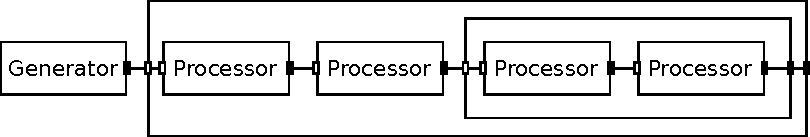
\includegraphics[width=\columnwidth]{fig/queue_model.pdf}
    \caption{Queue model for depth 3 and width 2.}
    \label{fig:queue_model}
\end{figure}

\begin{figure}
    \center
    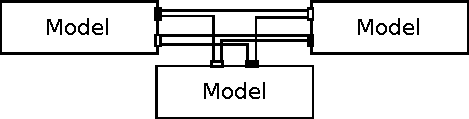
\includegraphics[width=\columnwidth]{fig/interconnect_model.pdf}
    \caption{HighInterconnect model for four models.}
    \label{fig:interconnect_model}
\end{figure}

\begin{figure}
    \center
    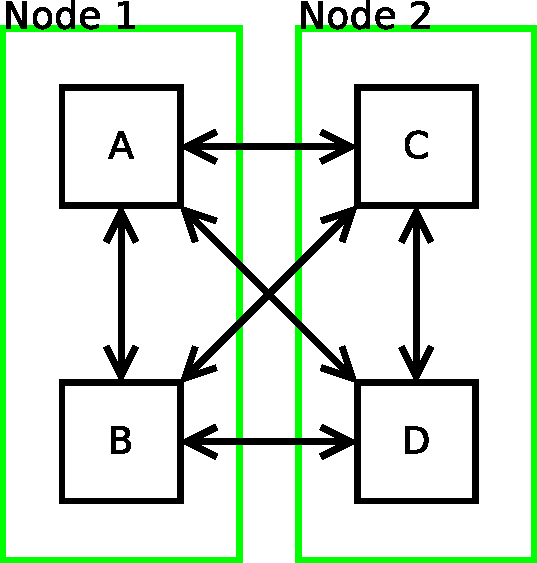
\includegraphics[width=0.5\columnwidth]{fig/phold_model.pdf}
    \caption{PHOLD model for four models, split over two nodes. In parallel simulation, each coupled model is simulated at a different node.}
    \label{fig:PHOLD_model}
\end{figure}

\subsection{Sequential Simulation Execution Time}
Despite our core contribution being mainly in the parallel simulation, we still value a comprehensive comparison of sequential simulation results.
First, and foremost, as parallel simulation results are tightly linked to the sequential simulation results: parallel simulation merely adds a synchronization layer over multiple, essentially sequential, simulation kernels.
Second, parallel simulation results are validated through the use of adevs.
To provide a more comprehensive comparison to adevs in the parallel simulation benchmarks, sequential simulation results need to be compared.
Only the Queue and HighInterconnect models are relevant for sequential simulation, so we will not touch upon the PHold model yet.

\subsubsection{Queue}
In the Queue model, we increase both the width and depth simultaneously, causing a quadratic growth in the number of atomic models.
As can be seen in Figure~\ref{fig:Queue_benchmark}, dxex considerably outperforms adevs.
Through careful analysis of profiling results, we determined that adevs spends much time while handling simulation messages, while this is mostly avoided in dxex's differently designed simulation algorithm.
Both simulation tools have similar complexities, though dxex is much faster thanks to its more efficient simulation control algorithms.

\begin{figure}
	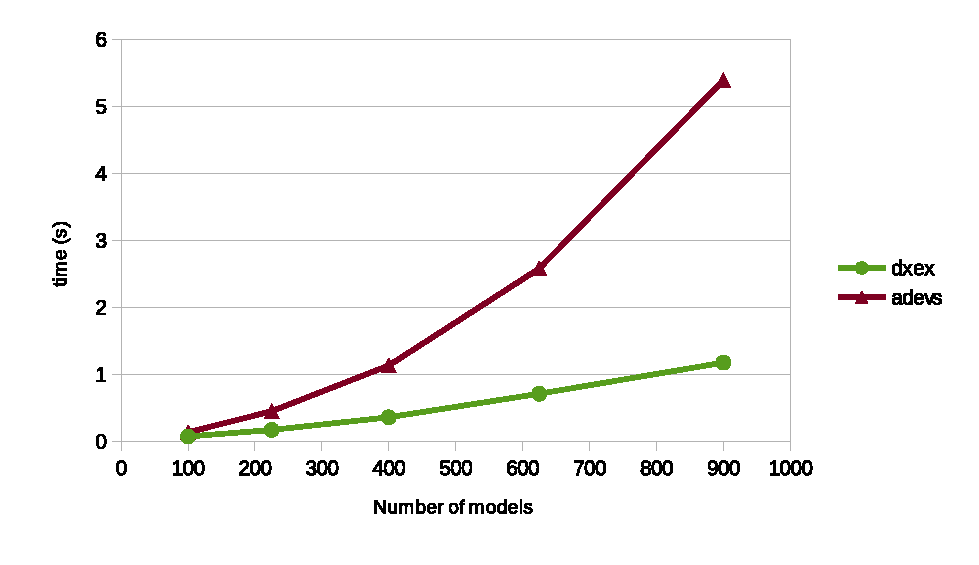
\includegraphics[width=\columnwidth]{fig/queue_sequential.eps}
	\caption{Queue benchmark results for sequential simulation.}
	\label{fig:Queue_benchmark}
\end{figure}

\subsubsection{HighInterconnect}
In the HighInterconnect model, we increase the number of atomic models, thus quadratically increasing the number of couplings.
As can be seen in Figure~\ref{fig:Interconnect_benchmark}, adevs now outperforms dxex by a fair margin.
Analysis showed that this slowdown is caused by the high amount of exchanged events: event creation is found to be much slower in dxex than it is in adevs, despite the use of memory pools in dxex.

\begin{figure}
	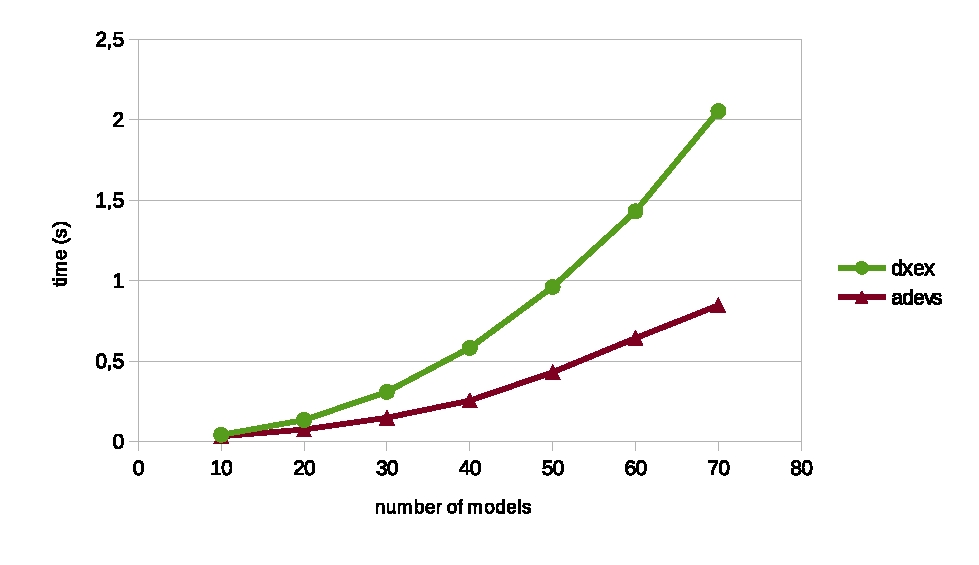
\includegraphics[width=\columnwidth]{fig/interconnect_sequential.eps}
	\caption{Interconnect benchmark results for sequential simulation.}
	\label{fig:Interconnect_benchmark}
\end{figure}

\subsection{Parallel Simulation Execution Time}
We now perform an analysis of parallel simulation execution times of our previously defined benchmarks.
For dxex, we mention results for both conservative and optimistic synchronization.
Since adevs supports only conservative synchronization, we don't mention optimistic synchronization results there.
All experiments were performed using up to six simulation nodes, and executed on a hexa-core machine.

We highlight two main results:
(1) dxex conservative synchronization is competitive with adevs;
(2) dxex optimistic synchronization is sometimes more efficient than conservative synchronization.
This shows that our contribution, offering both conservative and optimistic synchronization, is indeed beneficial for a general-purpose simulation tools.

\subsubsection{Queue}
In the Queue model, we allocate the chain of models such that each node is responsible for a series of connected models.
This minimizes the number of inter-node messages.
As the model is a queue, however, the last models will only activate later in the simulation.
Since these are allocated to separate nodes, some nodes will remain idle until simulation has progressed sufficiently far.

Similar to the sequential benchmarks, Figure~\ref{fig:queue_benchmark_parallel} shows that dxex again outperforms adevs, but now also in terms of speedup.
Results indicate that our implementation of conservative synchronization achieves much higher speedups than adevs.
This simulation is the ideal case for our conservative implementation, approaching near linear speedup.
In this case, conservative synchronization seems to be better than optimistic synchronization, at the cost of providing the lookahead.

\begin{figure}
	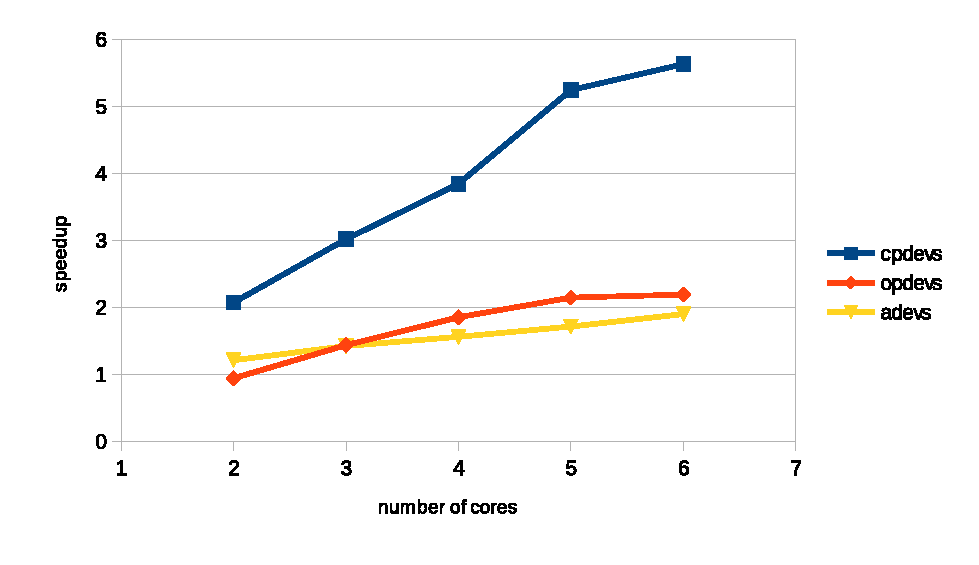
\includegraphics[width=\columnwidth]{fig/queue_parallel.eps}
	\caption{Queue benchmark results for parallel simulation of a model of fixed size.}
	\label{fig:queue_benchmark_parallel}
\end{figure}

\subsubsection{PHold}
In the Phold model, we first investigate the influence of the fraction of remote events on the speedup.
When remote events are rare, optimistic synchronization will rarely have to perform rollbacks, thus increasing performance.
With more common remote events, however, optimistic synchronization quickly slows down due to the frequent rollbacks.
Conservative synchronization, on the other hand, is mostly unconcerned with the number of remote events: the mere fact that a remote event can happen, causes it to block.
Even though a single synchronization protocol is always ideal in this case, it shows how different synchronization protocols respond differently to a changing model.
Adevs is significantly slower during conservative synchronization.
Analysis of profiling results shows that this was caused by exception handling within the adevs simulation kernel.

\begin{figure}
    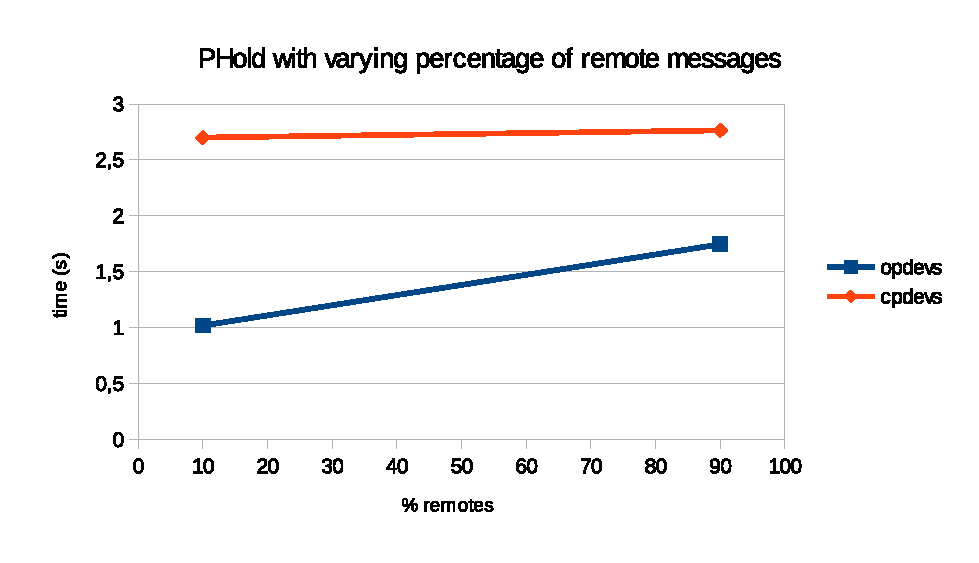
\includegraphics[width=\columnwidth]{fig/phold_remotes.eps}
    \caption{Phold benchmark results for parallel simulation using 6 cores, with varying fraction of remote events.}
\end{figure}

We further verify that our contribution fulfills our projected use case: a single model that can be tweaked to favor either conservative or optimistic synchronization.
We slightly modified the Phold benchmark, to include high-priority events.
Contrary to normal events, which offer a sufficiently large lookahead, high-priority events happen almost instantaneously, restricting lookahead to a very small value.
Even though normal events  occur most often, a conservative implementation always blocks until it can make guarantees.
An optimistic implementation, however, will simply go forward in simulation time and roll back the few times that these high-priority events happen.
This situation closely mimics the case made in the comparison between both synchronization algorithms by~\cite{FujimotoBook}.

Figure~\ref{fig:phold_priority} shows how simulation performance is influenced by the fraction of high-priority events.
If barely any high-priority events occur, conservative synchronization is penalized due to its excessive blocking, which often turned out to be unnecessary.
When many high-priority events occur, optimistic synchronization is penalized due to its mindless progression of simulation, which frequently needed to be reverted.
Results show that there is no single perfect synchronization algorithm for this model.
Depending on model configuration, either synchronization protocol might be better.
We have shown that our contribution is invaluable for high performance simulation: depending on the observed communication behaviour, modellers can use the most appropriate synchronization protocol.

\begin{figure}
    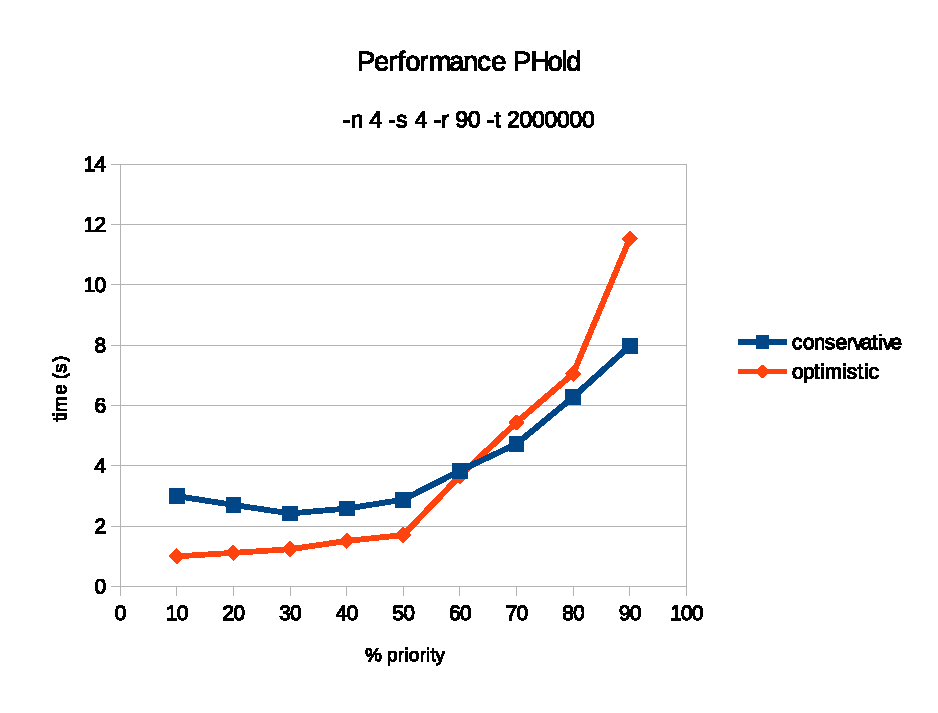
\includegraphics[width=\columnwidth]{fig/phold_voorlopig.eps}
    \caption{Phold benchmark results for parallel simulation using 6 cores, with varying amount of high-priority events.}
    \label{fig:phold_priority}
\end{figure}

\subsubsection{Interconnect}
In the Interconnect model, we determine how broadcast communication is supported across multiple nodes.
Results are shown in Figure~\ref{fig:interconnect_benchmark_parallel}
When the number of nodes increases, performance decreases due to increasing contention in conservative simulation and an increasing amount of reverts in optimistic. In this benchmark, all models depend on each other, negating any possible performance gain by executing the simulation in parallel.

\begin{figure}
    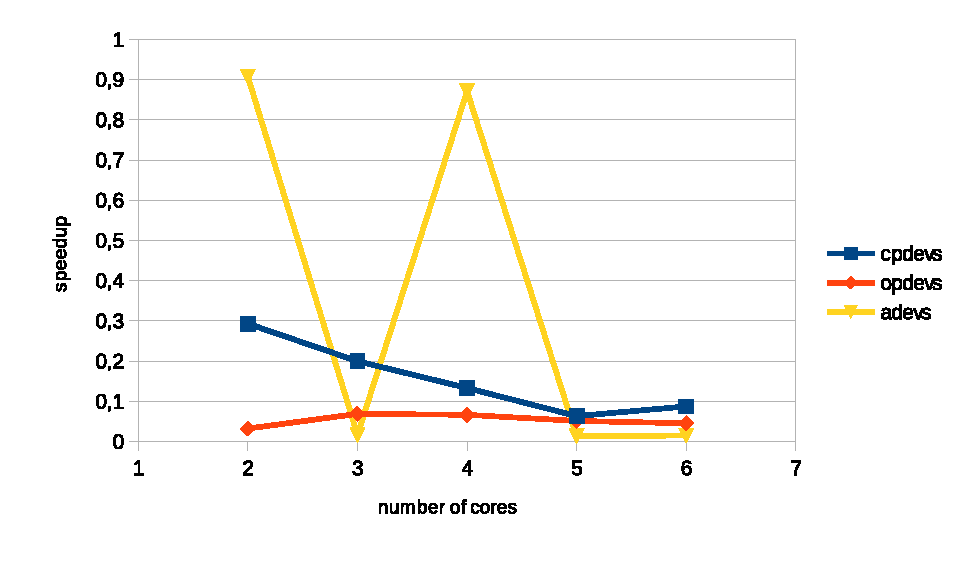
\includegraphics[width=\columnwidth]{fig/interconnect_parallel.eps}
    \caption{Interconnect benchmark results for parallel simulation.}
    \label{fig:interconnect_benchmark_parallel}
\end{figure}

\subsection{Memory Usage}
Apart from simulation execution time, memory usage during simulation is also of great importance.
While execution time only becomes a problem if it takes way too long, coming short only a bit of memory can make simulation infeasible.
We therefore also investigate memory usage of different synchronization protocols.

We do not tackle the problem of states that become too large for a single machine to hold.
This problem can be mitigated by distribution over multiple machines, which neither dxex or adevs support.
Comparison of memory usage should thus only be seen in the context of which models are feasible to be simulated by the tool.

\subsubsection{Remarks}
Both dxex and adevs use \texttt{tcmalloc} as memory allocator.
Additionally, dxex uses memory pools to further reduce the frequency of expensive system calls (\textit{e.g.}, malloc and free).
\texttt{tcmalloc} only gradually releases memory back to the OS, whereas our pools will not do so at all.
If memory has been allocated once, it is, at least from a performance point of view, better to keep that memory in the pool indefinitely.
Due to our motivation for memory usage analysis, we will only measure peak allocation.
Profiling is done using Valgrind's massif tool~\cite{Nethercote:2007:VFH:1273442.1250746}.

\subsubsection{Results}
Figure~\ref{fig:memory} shows the memory used by each different benchmark.
Results are in megabytes, and show the total memory footprint of the running application (\textit{i.e.}, text, stack, and heap).

Unsurprisingly, optimistic synchronization results show very high memory usage due to the saved states.
Note the logarithmic scale that was used for this reason.
Also, results for optimistic synchronization vary heavily depending on thread scheduling by the operating system, as this influences the drift between different nodes.
Comparing similar approaches though, we notice that dxex and adevs have very similar memory use.

Conservative simulation always uses more memory than sequential simulation, as is to be expected.
Additional memory is required for the multiple threads, but also to store all events that are processed simultaneously.

For the Phold benchmark, adevs using conservative synchronization took too long using our profiling tool, and was therefore aborted.
Therefore, no results are shown for adevs.

\begin{figure}
    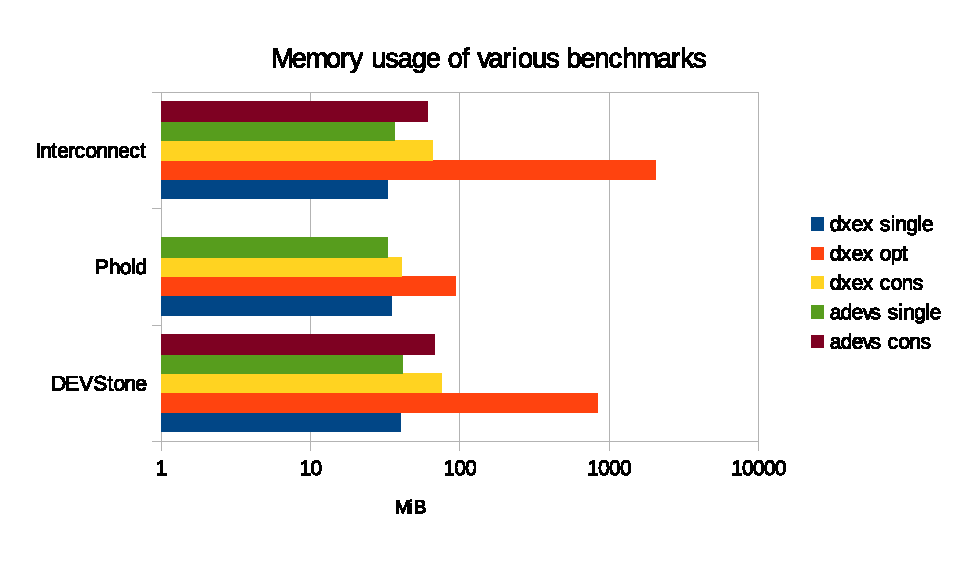
\includegraphics[width=\columnwidth]{fig/memory_voorlopig.eps}
    \caption{Memory usage results.}
    \label{fig:memory}
\end{figure}
